\section{Arquitetura de Grasews}\label{4-grasews-arquitetura}

%A ferramenta consiste de um sistema web que consome um conjunto de serviços disponibilizados por uma API (\textit{Application Programming Interface}). Utilizamos o \textit{Postgres}~\cite{POSTGRES-2019} como o sistema gerenciador de banco de dados (SGBD).
%Ambos foram hospedados na plataforma \textit{online} \textit{Microsoft Azure} (\textit{Cloud Computing Platform \& Services})~\cite{MICROSOFT-2019-AZURE}

Esta seção apresenta uma visão geral acerca da arquitetura de desenvolvimento de Grasews, juntamente com uma visão detalhada dos módulos da arquitetura e as integrações destes módulos.

\subsection{Visão Geral}\label{4-grasews-arquitetura-visao-geral}

O desenvolvimento de Grasews segue a abordagem de desenvolvimento \textit{Domain-Driven Design} (DDD)~\cite{EVANS-2004-DDD}. 
A \figurename~\ref{fig:grasews-architectural-projects} apresenta os módulos existentes na arquitetura de Grasews distribuídos nas camadas da abordagem DDD.

\begin{figure}[h]
    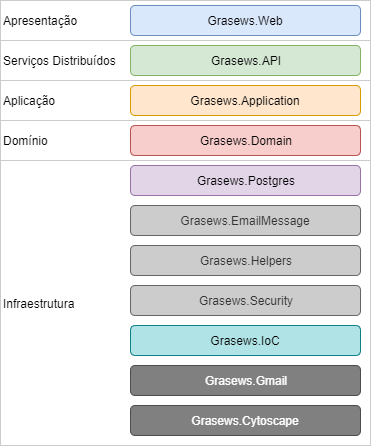
\includegraphics[scale=0.7]{4-grasews/imagens/grasews-architectural-projects.png}
    \centering
    \caption[Camadas e módulos da arquitetura da ferramenta Grasews]{\textbf{Camadas e módulos da arquitetura da ferramenta Grasews.}}
    \label{fig:grasews-architectural-projects}
\end{figure}

\newpage

A partir da abordagem DDD, a solução implementada consiste de cinco (5) camadas:

\begin{enumerate}

  \item
  \textit{\textbf{Apresentação}}:
  
  Esta camada de \textit{front-end} é composta pelo módulo \texttt{Grasews.Web}, que provê a interface gráfica de usuário (UI) da ferramenta.
  
  \item
  \textit{\textbf{Serviços Distribuídos}}:
  
  Esta camada é composta pelo módulo \texttt{Grasews.API}, que provê uma API para expor as funcionalidades do \textit{back-end} de Grasews. Esta API consiste de um conjunto de operações disponibilizadas por meio de serviços web RESTful. Todas as ações executadas por um usuário que necessitam interação com os demais módulos do lado servidor (\textit{back-end}) da aplicação são exclusivamente realizadas através da API.
  
  \item
  \textit{\textbf{Aplicação}}:
  
  Esta camada de \textit{back-end} é composta pelo módulo \texttt{Grasews.Application}, responsável por orquestrar as regras de negócio da aplicação.
  
  \item
  \textit{\textbf{Domínio}}:
  
  Esta camada de \textit{back-end} é composta pelo módulo \texttt{Grasews.Domain}, responsável por definir as regras de negócio da aplicação e as entidades de domínio do negócio. As regras de negócio são providas por meio de interfaces de desenvolvimento contidas neste módulo. Os demais módulos da aplicação seguem regras ditadas pelo módulo \texttt{Grasews.Domain}. A arquitetura de Grasews possui o seu desenvolvimento orientado a interfaces e não a implementações de classes. Tal característica facilita a substituição de um módulo da aplicação por outro módulo que, por exemplo, utiliza outra tecnologia diferente. Por exemplo, caso optemos por não usar mais o SGBD \textit{Postgres}, substituindo-o pelo SGBD \textit{Microsoft SQL Server}\cite{SQLSERVER-2019}, basta substituirmos o módulo \texttt{Grasews.Postgres} por, por exemplo, o módulo \texttt{Grasews.SqlServer}, o qual utilizaria as bibliotecas apropriadas para o acesso ao novo banco de dados. Adicionalmente, por meio das interfaces de  \texttt{Grasews.Domain}, garantimos que toda a aplicação funcione seguindo regras definidas pelo domínio (núcleo da aplicação).
  
  \item
  \textit{\textbf{Infraestrutura}}:
  
  Esta camada de \textit{back-end} é subdivida em três subcamadas de módulos: i) acesso a dados; ii) corte transversal; e iii) serviços externos.  A subcamada de acesso a dados é composta pelo módulo \texttt{Grasews.Postgres}, responsável por conectar a aplicação ao SGBD Postgres~\cite{POSTGRES-2019}. A subcamada de corte transversal é composta pelos módulos \texttt{Grasews.EmailMessage}, \texttt{Grasews.Helpers}, \texttt{Grasews.Security} e \texttt{Grasews.IoC}. O módulo \texttt{Grasews.EmailMessage} provê suporte à construção de mensagens de \textit{e-mail}. O módulo \texttt{Grasews.Helpers} provê suporte funcional às demais camadas e, consequentemente, aos demais módulos. Por exemplo, funcionalidades de suporte à leitura de XML, funcionalidades de suporte à manipulação de enumeradores e funcionalidades de suporte à requisições HTTP entre o \textit{front-end} e a API. O módulo \texttt{Grasews.Security} provê suporte à funcionalidades de segurança da aplicação. Por exemplo, funcionalidades de suporte à autenticação e permissões de um usuário. Finalmente, o módulo \texttt{Grasews.IoC} provê suporte funcional à inversão de controle (\textit{inversion of control} - IoC) e à injeção de dependências (\textit{dependency injection} - DI).
  
  A inversão de controle é uma técnica utilizada para reduzir o acoplamento entre objetos (classes) de uma arquitetura de \textit{software}. A arquitetura de um projeto pode ser severamente prejudicada quando tem-se um alto acoplamento, podendo tornar a sua manutenção custosa e até mesmo dificultar a sua evolução.
  
  A injeção de dependências é uma forma de se aplicar a inversão de controle, garantindo então um baixo acoplamento em um conjunto de classes. O padrão de injeção de dependência é baseado em abstrações das classes, por meio de classes abstratas ou interfaces de desenvolvimento. Segundo este padrão, o desenvolvimento é orientado à interface de uma classe ao invés de sua verdadeira implementação. A injeção de dependências de Grasews é feita por meio da injeção de objetos (dependências) por meio de construtores. Com isso, uma classe que necessita de instâncias de outras classes (dependências) obtém tais instâncias por meio da injeção destes objetos no construtor desta classe dependente.
  
  Por fim, a camada de serviços externos é composta pelos módulos \texttt{Grasews.Cytoscape} e \texttt{Grasews.Gmail}. O módulo de serviço externo \texttt{Grasews.Cytoscape} provê suporte à construção dos grafos WSDL e OWL da ferramenta. Este módulo utiliza a biblioteca \textit{Cytoscape.js}~\cite{CYTOSCAPE-2015}. Já o módulo de serviço externo \texttt{Grasews.Gmail} provê suporte ao envio de mensagens de \textit{e-mail} aos usuários por meio do serviço do \textit{Gmail}~\cite{GOOGLE-2019-GMAIL}.
  
\end{enumerate}
\subsection{Interações entre Módulos Grasews}\label{4-grasews-interacoes-modulos}

A \figurename~\ref{fig:grasews-architecture-simplified} apresenta uma visão geral das principais interações existentes entre os módulos Grasews. Uma seta preta e sólida representa as interações de um usuário com a aplicação. Uma linha azul, sólida e com setas sólidas nas duas extremidades representa interações entre os módulos utilizando objetos, i.e., instâncias de classes conforme a programação orientada a objetos. Uma linha rosa e tracejada representa injeções de dependências. Uma linha verde e tracejada representa implementações de interfaces de desenvolvimento. A extremidade com a seta verde e vazia indica a definição das interfaces contidas em \texttt{Grasews.Domain}, enquanto que a extremidade com o círculo verde e sólido indica um módulo que implementa uma interface definida em \texttt{Grasews.Domain}. Uma seta vermelha e tracejada indica interações realizadas por meio do protocolo HTTP entre os módulos da aplicação. Por fim, uma seta laranja e tracejada representa eventos assíncronos. A extremidade com o círculo laranja e vazio representa a origem dos eventos assíncronos, enquanto que a extremidade com a seta laranja e vazia indica o módulo onde os eventos assíncronos são notificados.

\begin{figure}[h]
    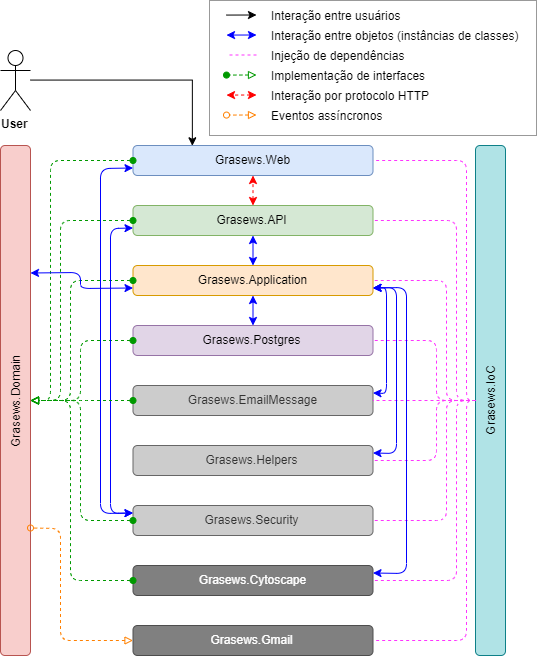
\includegraphics[scale=0.55]{4-grasews/imagens/grasews-architecture-simplified.png}
    \centering
    \caption[Arquitetura da ferramenta Grasews]{\textbf{Arquitetura da ferramenta Grasews.}}
    \label{fig:grasews-architecture-simplified}
\end{figure}

De forma resumida e simplificada, o fluxo da aplicação segue da seguinte forma: O usuário interage com o módulo \texttt{Grasews.Web}, o qual se comunica com \texttt{Grasews.API} por meio de requisições HTTP. Tanto \texttt{Grasews.Web} quanto \texttt{Grasews.API} utilizam funcionalidades providas por objetos de \texttt{Grasews.Security}. \texttt{Grasews.API} consome serviços providos por \texttt{Grasews.Application}, o qual orquestra o fluxo de trabalho conforme as regras de negócio da aplicação. Neste sentido, \texttt{Grasews.Application} é responsável por manipular objetos das entidades de domínio da aplicação juntamente com funcionalidades de apoio providas por \texttt{Grasews.Helpers}. Adicionalmente, \texttt{Grasews.Application} utiliza funcionalidades providas por \texttt{Grasews.Cytoscape}, para a manipulação de elementos do grafo, e funcionalidades providas por \texttt{Grasews.EmailMessage}, para a construção de mensagens de \textit{e-mail}. Juntamente com \texttt{Grasews.Gmail}, \texttt{Grasews.Application} invoca um evento assíncrono de \texttt{Grasews.Domain} para que a mensagem de \textit{e-mail}, previamente construída por \texttt{Grasews.EmailMessage}, seja enviada para um usuário. \texttt{Grasews.IoC} provê a injeção de dependências para todos os demais módulos da arquitetura.
\subsection{Interações Detalhadas entre Módulos de Grasews}\label{4-grasews-interacoes-detalhadas-modulos}

A \figurename~\ref{fig:grasews-architecture-detailed} detalha as principais interações dos módulos da arquitetura de Grasews. O fluxo da aplicação inicia-se com um usuário interagindo com a interface gráfica da aplicação por meio do módulo  \texttt{Grasews.Web} (à esquerda, na cor azul). \texttt{Grasews.Web} foi desenvolvido utilizando o padrão de arquitetura de desenvolvimento MVC e, portanto, seus principais componentes são representados por \texttt{Models}, \texttt{Views} e \texttt{Controllers}. Um usuário interage com um componente \texttt{View} que, por sua vez, utiliza um objeto modelo definido por um componente \texttt{Model}. A ações de um usuário resultam em eventos controlados por um componente \texttt{Controller}. O componente \texttt{Startup} é responsável por requisitar ao componente \texttt{SimpleInjectorBootstrap} o controle de dependências da aplicação. \texttt{SimpleInjectorBootstrap} (canto inferior, na cor ciano), do módulo \texttt{Grasews.IoC}, é responsável por criar um repositório de referências a objetos (classes) que serão necessários e utilizados por toda a aplicação. Estes objetos tornam-se disponíveis aos demais componentes da aplicação por meio da injeção de dependências realizada nos construtores destes demais componentes. Por fim, um componente de \texttt{Controller} utiliza o componente \texttt{RestClient} para que uma nova requisição seja feita à API da aplicação. O componente \texttt{RestClient} (canto superior, na cor vermelha) é provido pelo módulo \texttt{Grasews.Helpers} (canto superior, na cor cinza claro).

\begin{landscape}
    \begin{figure}[h]
        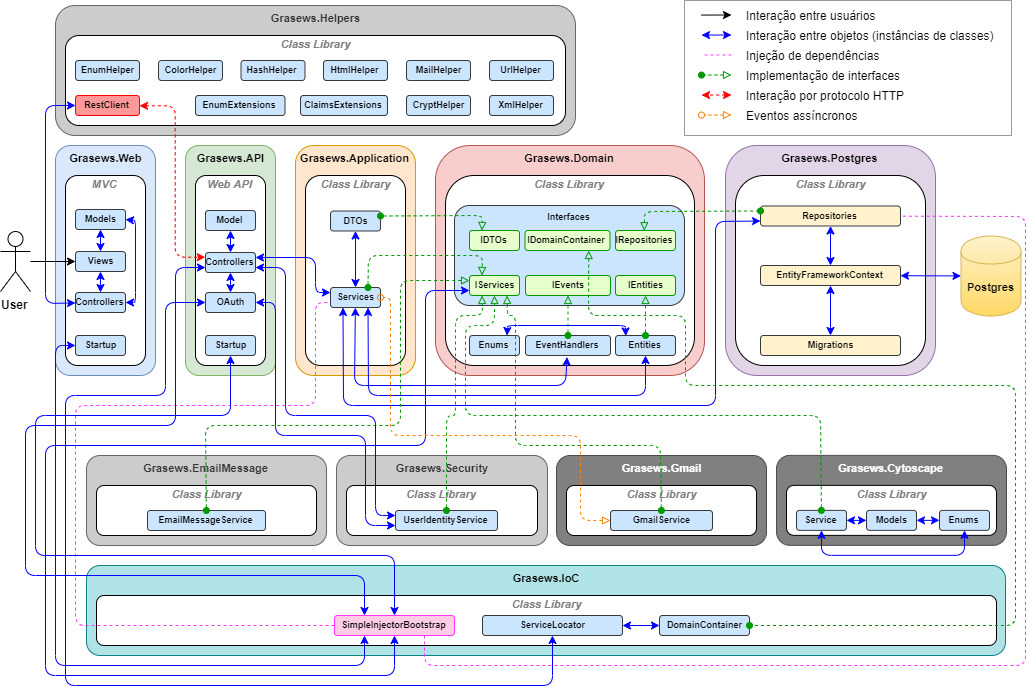
\includegraphics[scale=0.6]{4-grasews/imagens/grasews-architecture-detailed.png}
        \centering
        \caption[Arquitetura do Grasews de forma detalhada]{\textbf{Arquitetura do Grasews de forma detalhada.}}
        \label{fig:grasews-architecture-detailed}
    \end{figure}
\end{landscape}

A API da aplicação é provida pelo módulo \texttt{Grasews.API} (centro à esquerda, na cor verde). Os principais componentes deste módulo são os \texttt{Controllers} e os \texttt{Models}. As requisições originadas de \texttt{Grasews.Web} são gerenciadas por um \texttt{Controller} da API. Tais requisições são repassadas aos serviços do módulo \texttt{Grasews.Application}. Adicionalmente, \texttt{Grasews.API} contém o componente \texttt{Startup}, que assim como no módulo \texttt{Grasews.Web}, este componente é responsável por requisitar o registro de dependências ao módulo \texttt{Grasews.IoC}. Por fim, todos as requisições realizadas para \texttt{Grasews.API} são protegidas. Para realizar uma ação na ferramenta, o usuário deve ser autenticado pelo componente \texttt{OAuth}. Este componente é responsável por validar as credenciais de um usuário, permitindo o uso das funcionalidades da ferramenta, tanto por meio do módulo \texttt{Grasews.Web} quanto do módulo \texttt{Grasews.API}. O componente \texttt{OAuth} utiliza recursos providos por \texttt{UserIdentityService}, do módulo \texttt{Grasews.Security}, localizado no centro inferior do diagrama, na cor cinza claro. Adicionalmente, \texttt{OAuth} utiliza o componente \texttt{ServiceLocator} para obter instâncias de classes que ainda não foram introduzidas no contexto da aplicação pelo componente \texttt{SimpleInjectorBootstrap}. Isso ocorre pelo fato do componente \texttt{OAuth} ser instanciado no início do ciclo da vida da aplicação e não permitir que seu construtor tenha parâmetros de entrada, fator este que possibilita a injeção de dependências. \texttt{ServiceLocator} é auxiliado pelo componente \texttt{DomainContainer}, que atua como um repositório de objetos da aplicação.

O módulo \texttt{Grasews.Application} é representado simplificadamente por meio dos componentes \texttt{Services} e \texttt{DTOs} (\textit{Data Transfer Objects}). As classes que compõem os serviços (\texttt{Services}) são responsáveis por orquestrar todas as requisições originadas do módulo \texttt{Grasews.API}. Requisições realizadas ao módulo \texttt{Grasews.Application} resultam na utilização de objetos das camadas inferiores, como, por exemplo, a criação de instâncias de entidades de domínio, de \texttt{Grasews.Domain}, ou o consumo de métodos de classes de acesso a dados, denominados repositórios, de \texttt{Grasews.Postgres}. Os parâmetros de entrada e de saída de serviços do módulo \texttt{Grasews.Application} variam entre tipos simples, e.g., \textit{int} e \textit{string}, instâncias de entidades de domínio ou então instâncias de um \texttt{DTO}. Nenhum objeto de um tipo de \texttt{Model} de \texttt{Grasews.API} é transferido para \texttt{Grasews.Application}. Os \texttt{Controllers} de \texttt{Grasews.API} são responsáveis por converter seus objetos de tipos de  \texttt{Models} para objetos de tipo de uma entidade de domínio ou então de tipo de um \texttt{DTO}. Desta forma, obtém-se uma melhor segregação do escopo de objetos de cada módulo e, consequentemente, um maior desacoplamento entre os módulos, tornando um módulo o mais autossuficiente possível.

O módulo \texttt{Grasews.Domain} (centro, na cor salmão) contém todas as interfaces (na cor verde claro) de desenvolvimento que são implementadas pelos demais módulos da aplicação. Adicionalmente, \texttt{Grasews.Domain} é responsável por definir as entidades do domínio de negócio da aplicação, representadas pelo componente \texttt{Entities} (na cor azul). Uma entidade geralmente representa uma tabela no banco de dados. Por meio do módulo \texttt{Grasews.Postgres}, estas entidades e suas propriedades são mapeadas para tabelas e colunas do banco de dados, respectivamente. Por fim, \texttt{Grasews.Domain} possui componentes responsáveis por controlar eventos assíncronos. Eventos assíncronos são funcionalidades que podem ser executadas independentemente do fluxo da aplicação, pois não geram dependências para a aplicação. Por exemplo, o envio de um \textit{e-mail} para um usuário pode ser executado de forma assíncrona. Os componentes responsáveis pela implementação do controle de eventos assíncronos são os \texttt{EventHandlers} e as interfaces de \texttt{IEvents}.

O módulo \texttt{Grasews.Postgres} (centro à esquerda, na cor lilás) é responsável por realizar o acesso da aplicação ao banco de dados. Seus principais componentes são os repositórios (\texttt{Repositories}) e o contexto do banco de dados implementado pelo uso do \textit{Microsoft Entity Framework}. O contexto do banco de dados é representado por \texttt{EntityFrameworkContext}. Todas as ações executadas em Grasews que necessitam acesso ao banco de dados são realizadas pelos repositórios. Os repositórios implementam interfaces definidas no módulo \texttt{Grasews.Domain}. Grasews utiliza o SGBD \textit{Postgres} (centro à esquerda, na cor amarelo). Adicionalmente, toda a estrutura de banco de dados de Grasews foi gerada automaticamente por meio do componente \texttt{Migrations} com base nas classes de entidades de domínio existentes no módulo \texttt{Grasews.Domain}. \texttt{Migrations} permite que alterações no modelo do código sejam feitas e depois sejam propagadas no banco de dados.

O módulo \texttt{Grasews.Helpers} (canto superior, na cor cinza claro) possui componentes com funcionalidades que dão suporte a todos os demais módulos de Grasews. Este módulo é composto por diversos componentes com variados propósitos a fim de auxiliar demais objetos da arquitetura da ferramenta. Por fim, o módulo \texttt{Grasews.Cytoscape} (canto inferior direito, na cor cinza escuro) é responsável por manipular nós e arestas do grafo de Grasews. Este módulo foi desenvolvido baseado nas funcionalidades e modelos necessários da biblioteca de desenvolvimento \texttt{Cytoscape.js}, utilizada pelo módulo \texttt{Grasews.Web} para o desenvolvimento dos grafos na interface gráfica de usuário da ferramenta. Os principais componentes de \texttt{Grasews.Cytoscape} são \texttt{Service}, contendo os métodos para manipulação dos elementos (modelos) do grafo, e \texttt{Models}, contendo os tipos de dados necessários para a representação de elementos no grafo, como, por exemplo, nós, arestas e propriedades visuais.